\begin{frame}{Le péril IA ? La bataille des pionniers}
\begin{block}{}
    \textbf{\textrightarrow{}} Pétition \textit{Pause Giant AI Experiments: An Open Letter} en janvier 2023. Parmi les signataires: Elon Musk, Yoshua Bengio ou encore Steve Wauzniak.\\
\small
\url{https://en.wikipedia.org/wiki/Pause_Giant_AI_Experiments:_An_Open_Letter}
\end{block}
\vspace{10mm}

\centering
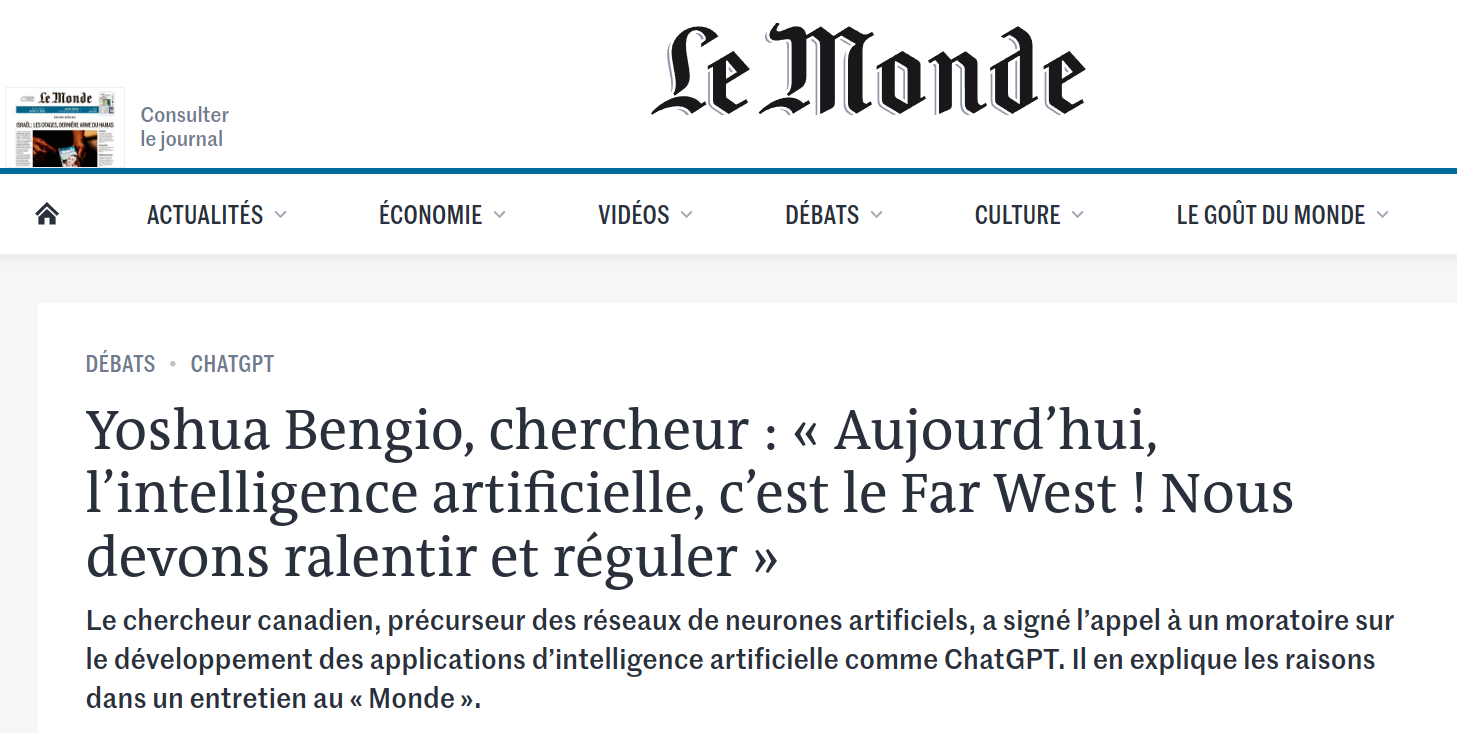
\includegraphics[width=0.45\textwidth]{04_Axe1_IAG/Images/Bengio.png}
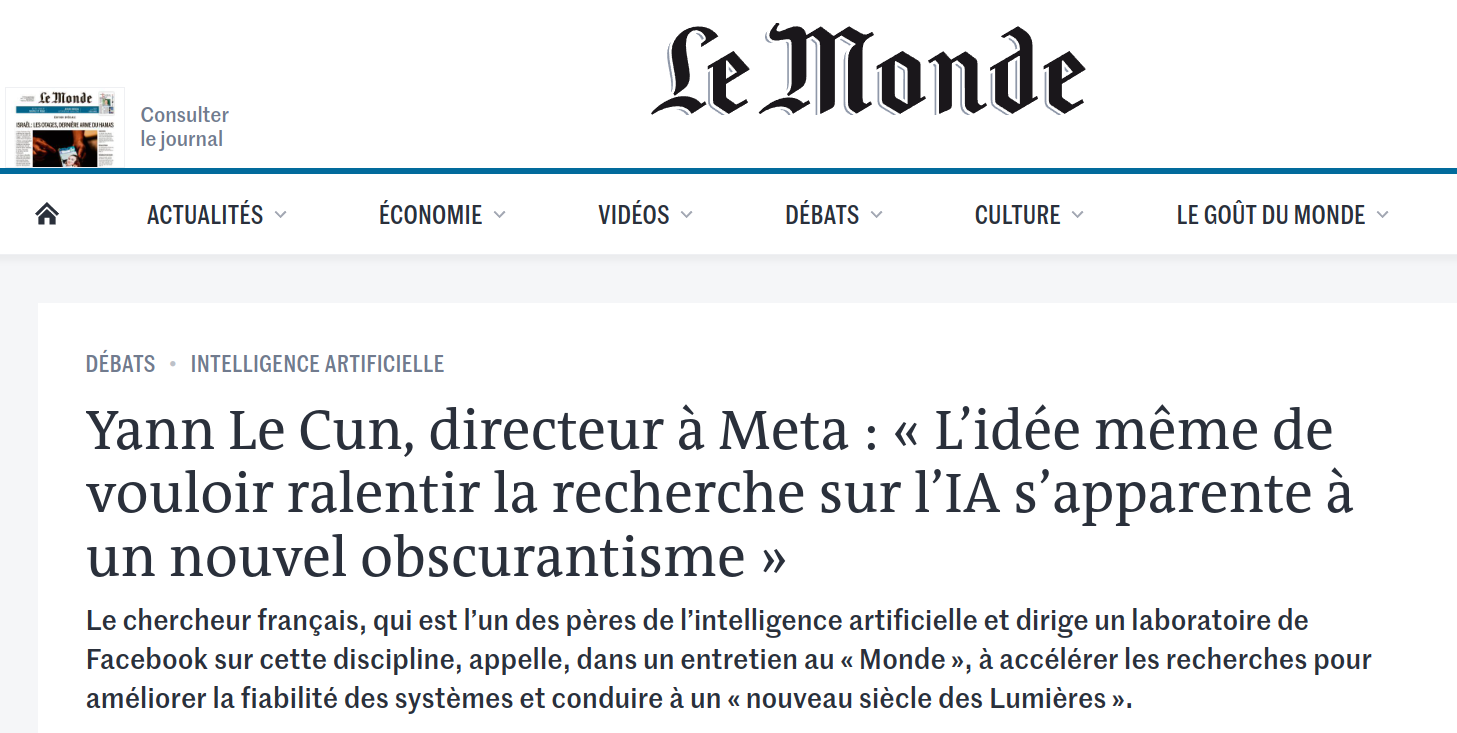
\includegraphics[width=0.45\textwidth]{04_Axe1_IAG/Images/LeCun.png}
\end{frame}

\begin{frame}{Le péril IA ? La bataille des pionniers}
\begin{columns}[T,onlytextwidth]
\column{0.50\linewidth}
\small
Yoshua Bengio, Yann Le Cun et Geoffrey Hinton ont publié ensemble l'article le plus cité dans le domaine des IA 

\column{0.50\linewidth}
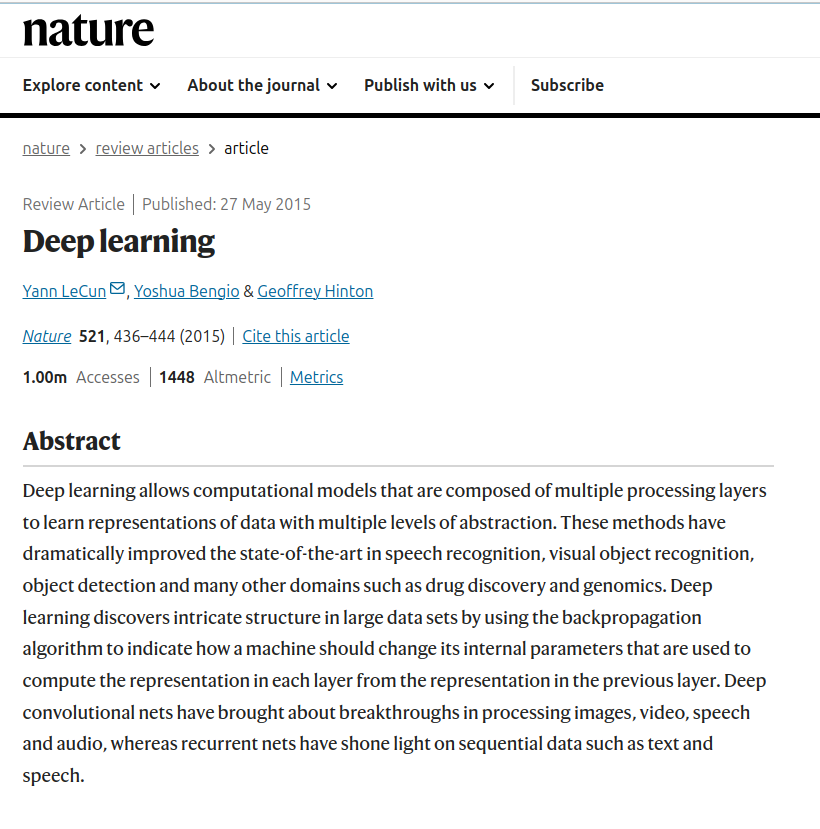
\includegraphics[width=0.80\textwidth]{04_Axe1_IAG/Images/articleIABengio-LeCun.png}
\end{columns}
\end{frame}

\begin{frame}{Le péril IA ? La bataille des pionniers}
\begin{block}{}
    Dans l'article du monde, Yoshua Bengio écrit:\\
    \vspace{3mm}
    \centering
    {\small \textit{"Les résultats restent imprévisibles, et nous ne comprenons pas parfaitement le fonctionnement de ce processus très complexe. Cela pose des questions de sécurité, de transparence, de fiabilité. On s’aperçoit très vite que ces systèmes inventent parfois des réponses, qu’ils peuvent aller dans une direction que n’ont pas choisie les programmeurs. La seule façon de les réorienter, c’est de les récompenser lorsque la réponse est pertinente. Depuis des mois, les concepteurs de ChatGPT travaillent à parer les coups, mais ce n’est pas suffisant."}}\\
\end{block}
\vspace{5mm}
\textrightarrow{} Manque de compréhension sur le fonctionnement de l'IA.\\
\textrightarrow{} Une question \textbf{éthique}.
\end{frame}

\begin{frame}{Le péril IA ? La bataille des pionniers}
\begin{block}{}
    A l'inverse, Yann Le Cun écrit:\\
    \vspace{3mm}
\centering
\small
\textit{"Ces capacités donnent l’impression que le système est intelligent, mais en fait elles restent superficielles. ChatGPT n’est pas intelligent comme peut l’être un humain. C’est un outil de prédiction, qui associe entre eux des mots apparaissant de façon la plus probable dans le corpus qui a servi à l’entraîner, afin de continuer un texte. [...] Ce sont des outils très utiles pour accélérer l’écriture de textes, en particulier de code informatique. Ils peuvent améliorer la productivité de nombreux professionnels, comme les programmeurs, ou les médecins qui veulent rédiger plus vite leurs comptes rendus de consultations. Il faut seulement informer les utilisateurs des limites de l’application : on ne peut pas s’en servir comme moteurs de recherche, ni se reposer sur les informations qu’elle produit sans les vérifier."}
\end{block}
\vspace{5mm}
\textrightarrow{} Selon lui, l'IA peut "conduire à une renaissance de l'humanité, un nouveau siècle des Lumières".
\end{frame}

\begin{frame}{Le péril IA ? La bataille des pionniers}
    \centering
    
\includegraphics[width=7cm]{04_Axe1_IAG/Images/The_Cake_is_a_Lie.jpg}
\end{frame}
\begin{frame}{Au fait, c'est quoi les IAG?}
\begin{block}{}
    \textbf{IAG (Intelligence artificielle générative)=} désignent des technologies de création de contenu, de génération de contenus (texte, images, sons), aujourd'hui implémentées dans des outils grand public : copilot, chatGPT, etc.
\end{block}
\vspace{3mm}
\centering
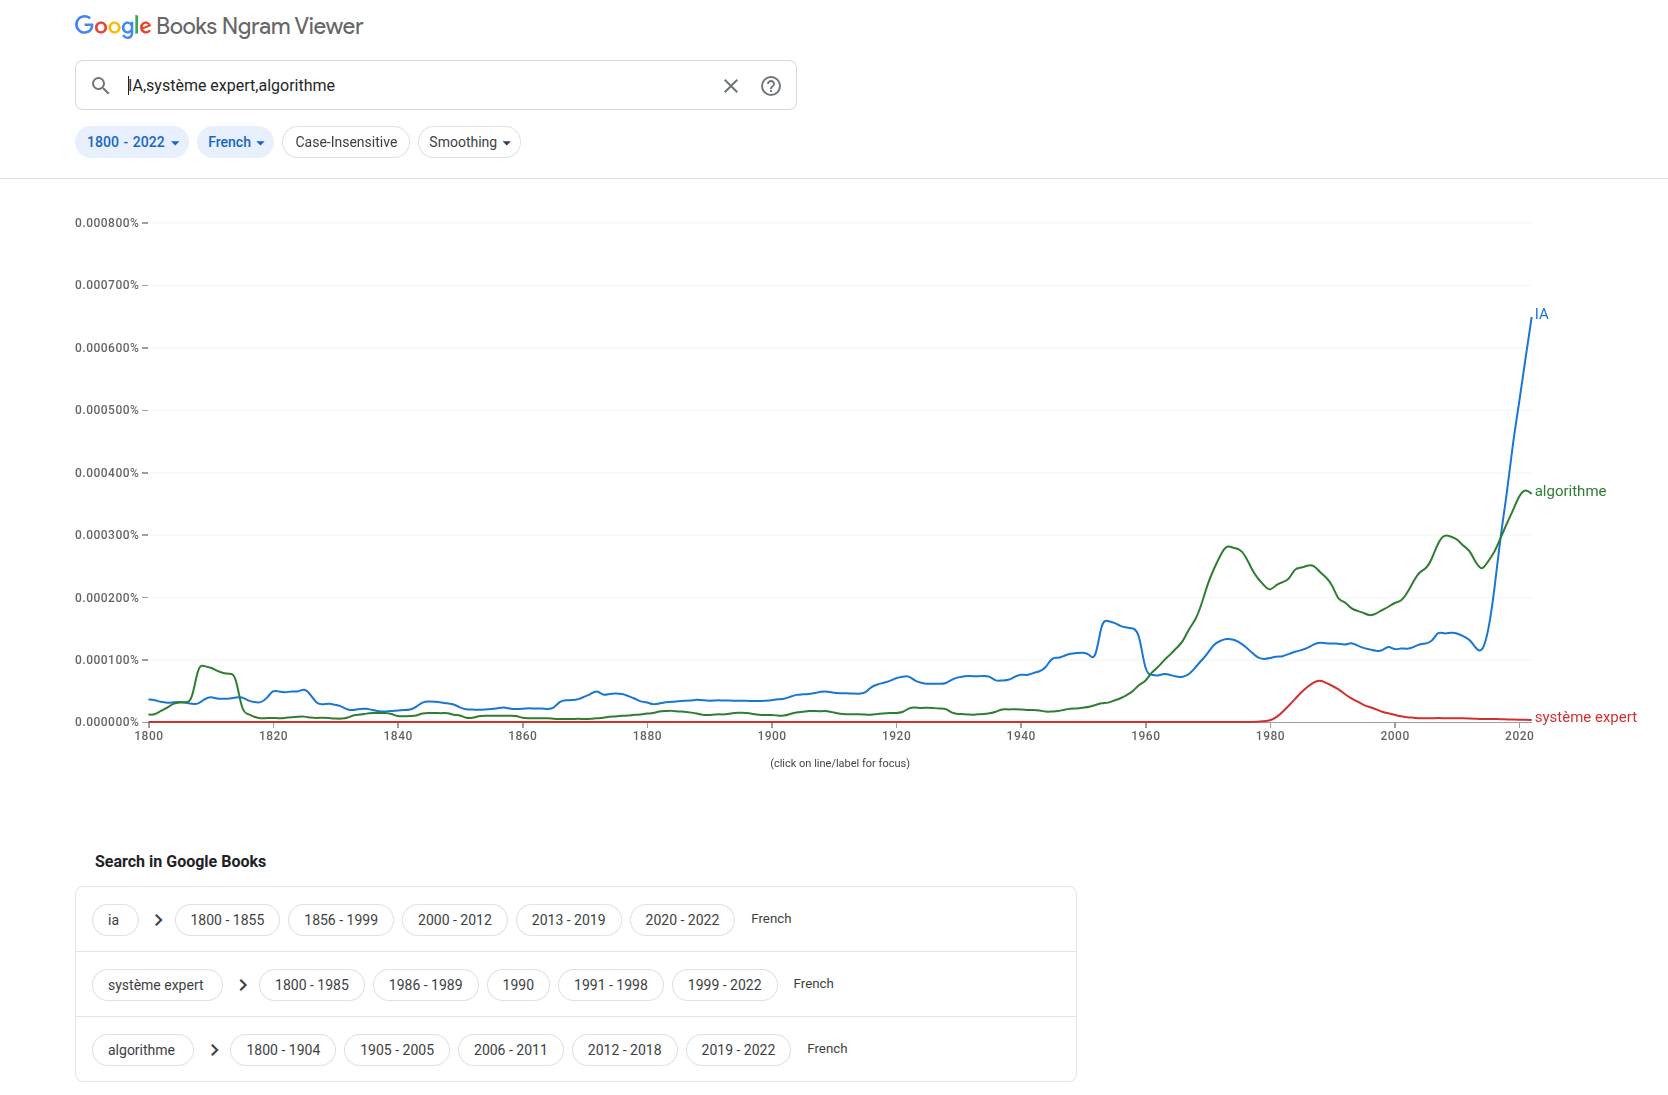
\includegraphics[width=0.65\textwidth]{04_Axe1_IAG/Images/googleNgramIA.png}
\end{frame}

\begin{frame}{"Intelligence artificielle"
une expression problématique et polémique}

\centering
\textbf{Qu'est-ce que l'intelligence?}

\end{frame}

\begin{frame}{Générative ?
}
\begin{block}{}
    \begin{itemize}
        \item Automatiser la production du texte
\item Le mythe du texte qui s'écrit tout seul
\item Une quête formaliste, poétique, ludique...\\
...qui n'a pas attendu ChatGPT !
    \end{itemize}
\end{block}

Rappel: les générateurs de texte=programme qui crée du texte à partir d’un ensemble de règles qui constituent une grammaire et d’un ensemble d’éléments préconstruits qui forment un dictionnaire. 

\end{frame}

\begin{frame}{Les générateurs combinatoires et automatiques}
Repose initialement sur un principe \textbf{combinatoire}.\\
\vspace{5mm}
\textbf{Un générateur combinatoire} = générateur de texte qui combine selon des règles algorithmiques spécifiques des fragments de textes préconstruits. Le générateur va ainsi tenter d’épuiser toutes les possibilités d’une structure à partir de différentes combinaisons des fragments entre eux.
\end{frame}

\begin{frame}{Atelier : étudier la modélisation de l'échange épistolaire amoureux chez Christopher Stratchey}
\centering

\includegraphics[width=0.40\textwidth]{04_Axe1_IAG/Images/atelier-love-letters.png}
\end{frame}

\begin{frame}{Oeuvres génératives}
    \centering
    {\small
    \textit{Ce qui m’intéresse dans la génération, ce n’est pas le texte qui s’affiche. Ce texte-là est un moment comme un autre, on s’en fout. […] Ce qui m’intéresse, c’est cette capacité à produire à l’infini et à générer un univers que je ne suis pas capable de faire. C’est donc un autre substitut qui transmet une pensée qui dit. Peut-être est-ce un fantasme d’éternité.}}\\
\textbf{Jean-Pierre Balpe
\textit{Oeuvre dans un paradigme "contemporain"} (emprunté à l'art contemporain)}

\end{frame}